%%%%%%%%%%%%%%%%%%%%%%%%%%%%%%%%%%%%%%%%%%%%%%%%%%%%%%%%%%%%%%%%%%%%%%%%%
% This file is part of the LaTeX sources of the OMDoc 1.2 specifiation
% Copyright (c) 2006 Michael Kohlhase
% This work is licensed by the Creative Commons Share-Alike license
% see http://creativecommons.org/licenses/by-sa/2.5/ for details
\svnInfo $Id: processing.tex 6154 2006-10-03 11:31:31Z  $
\svnKeyword $HeadURL: https://svn.omdoc.org/repos/omdoc/branches/omdoc-1.2/doc/spec/processing.tex $
%%%%%%%%%%%%%%%%%%%%%%%%%%%%%%%%%%%%%%%%%%%%%%%%%%%%%%%%%%%%%%%%%%%%%%%%%

\begin{tchapter}[id=transform-xsl,short=Transforming OMDoc]{Transforming OMDoc by XSLT Style Sheets}

In the introduction we have stated that one of the design intentions behind
{\omdoc} is to separate content from presentation, and leave the latter to the
user. In this section, we will briefly touch upon presentation issues. The
technical side of this is simple: {\omdoc} documents are regular {\xml} documents
that can be processed by {\xslt} {\indextoo{style sheet}s}~\cite{Clark:xslt99} to
produce the desired output formats. There are several high-quality {\xslt}
transformers freely available including {\snippetin{saxon}}~\cite{saxon_web},
{\snippetin{xalan}}~\cite{xalan_web}, and {\snippetin{xsltproc}}\cite{xsltproc_web}.
Moreover, {\xslt} is natively supported by the newest versions of the
{\indextoo{browser}}s {\msie}\index{internet@{\msie}}~\cite{ie_web} and
{\mozilla}~\cite{mozilla_web}.

{\xslt} style sheets can be used for several tasks in maintaining {\omdoc}, such as for
instance converting other {\xml}-based input formats into {\omdoc} (e.g.
{\snippetin{cd2omdoc.xsl}} for converting {\openmath} content dictionaries\index{content
  dictionary} into {\omdoc} format), or migrating between different versions of {\omdoc}
e.g. the style sheet {\snippetin{omdoc1.1adapt1.2.xsl}} that operationalizes all the
syntax changes from {\vomdoc{1.1}} to version 1.2 (see {\myappchapref{changelog}} for a
tabulation).  We will now review a set of {\xslt} style sheets for {\omdoc}, they can be
found in the {\omdoc} distribution (see {\mysecref{distribution}}) or on the web
at~\cite{OMDocXSL:URL}.

\begin{tsection}[id=extract-link-xslt]{Extracting and Linking XSLT Templates}

One of the main goals of content markup for mathematical documents is to be
independent of the output format. In {\mychapref{pres}}, we have specified the
conceptual infrastructure provided by the {\omdoc} language, in this section we
will discuss the software infrastructure needed to transform {\omdoc} documents
into various formats.

The {\element{presentation}} elements for symbols in {\openmath} or {\cmathml}
formulae allow a declarative specification of the result of transforming
expressions involving these symbols into various formats. To use this information
in {\xslt} style sheets, the content of {\element{presentation}} elements must be
transformed into {\xslt} templates, and these must be linked into the generic
transformation style sheet. The {\omdoc} distribution provides two
meta-style-sheets for these tasks.

The first one --- {\snippetin{expres.xsl}} --- compiles the content of the
{\element{presentation}} and {\element{omstyle}} elements in the source file into {\xslt}
templates\index{template!{\snippet{xslt}}}. The style sheet takes the parameter
{\snippetin{report-errors}}, which is set to '{\snippet{no}}' by default; setting it to
'{\snippet{yes}}' will enable more verbose error reports. The {\omdoc} distribution
provides {\unix} {\snippetin{Makefiles}} that specify the target
{\snippet{\llquote{base}-tmpl.xsl}} for each {\omdoc} file
{\snippet{\llquote{base}.omdoc}}, so that the templates file can be generated by typing
{\snippet{make \llquote{base}-tmpl.xsl}}. Note that {\snippetin{expres.xsl}} follows the
references in the {\element{ref}} elements (it {\element{ref}}-normalizes the document see
{\mysecref{sharing}}) before it generates the templates\footnote{In the current
  implementation, {\snippet{expres.xsl}} generates one large template that combines the
  {\xslt} code for all target formats. This simplifies the treatment of the default
  presentations as requested by the specification in {\mysecref{presentation}}, but
  hampers mixing presentation information from multiple sources. An implementation based
  on modes would probably have advantages in this direction in the long run.}.

The second style sheet --- {\snippetin{exincl.xsl}} --- generates link table for a
specific {\omdoc} document. This style sheet {\element{ref}}-normalizes the document and
outputs an {\xslt} style sheet that includes all the necessary template
files. {\snippetin{expres.xsl}} takes two parameters: {\snippet{self}} is the name of the
source file name itself\footnote{For some reason {\xslt} processors do not provide access
  to this information portably.}. The {\snippetin{Makefiles}} in the {\omdoc} distribution
specify the target {\snippet{\llquote{base}-incl.xsl}}, so that the link table can be
generated by typing {\snippet{make \llquote{base}-incl.xsl}}.

Let us now consider the example scenario in {\myfigref{omdoc_presentation}}: Given an
{\omdoc} document {\snippet{\llquote{document}.omdoc}} that uses symbols from theories
{\snippet{a}}, {\snippet{b}}, {\snippet{c}}, {\snippet{d}}, and {\snippet{e}} which are
provided by the {\omdoc} documents {\snippet{\llquote{background}.omdoc}},
{\snippet{\llquote{special}.omdoc}} and {\snippet{\llquote{local}.omdoc}}, we need to
generate the template files {\snippet{\llquote{background}-tmpl.xsl}},
{\snippet{\llquote{special}-tmpl.xsl}}, and {\snippet{\llquote{local}-tmpl.xsl}} (via
{\snippetin{expres.xsl}}) as well as {\snippet{\llquote{document}-incl.xsl}} (via
{\snippetin{exincl.xsl}}).  Now it is only necessary to include the link table
{\snippet{\llquote{document}-incl.xsl}} into a generic transformation style sheet to
specialize it with the notation information specified in the {\element{presentation}}
elements in theories {\snippet{a}}, {\snippet{b}}, {\snippet{c}}, {\snippet{d}}, and
{\snippet{e}}.

The transformation architecture based on the {\snippet{Makefiles}} provided with the
{\omdoc} distribution does the linking by creating a specialized style sheet
{\snippet{\llquote{document}2html.xsl}} that simply includes the generic {\omdoc}
transformation style sheet {\snippet{omdoc2html.xsl}} (see {\mysecref{omdoc2pres}}), and
the style sheet {\snippet{\llquote{document}-incl.xsl}}. Changing this simple control
style sheet allows to add site- or language-specific templates (by adding them directly or
including respective style sheets).  An analogous processing path leads
{\snippet{\llquote{document}.tex}} using {\snippet{omdoc2tex.xsl}} and from there to PDF
using tools like {\snippet{pdflatex}}.

\begin{myfig}{omdoc_presentation}{The {\omdoc} presentation Process}
  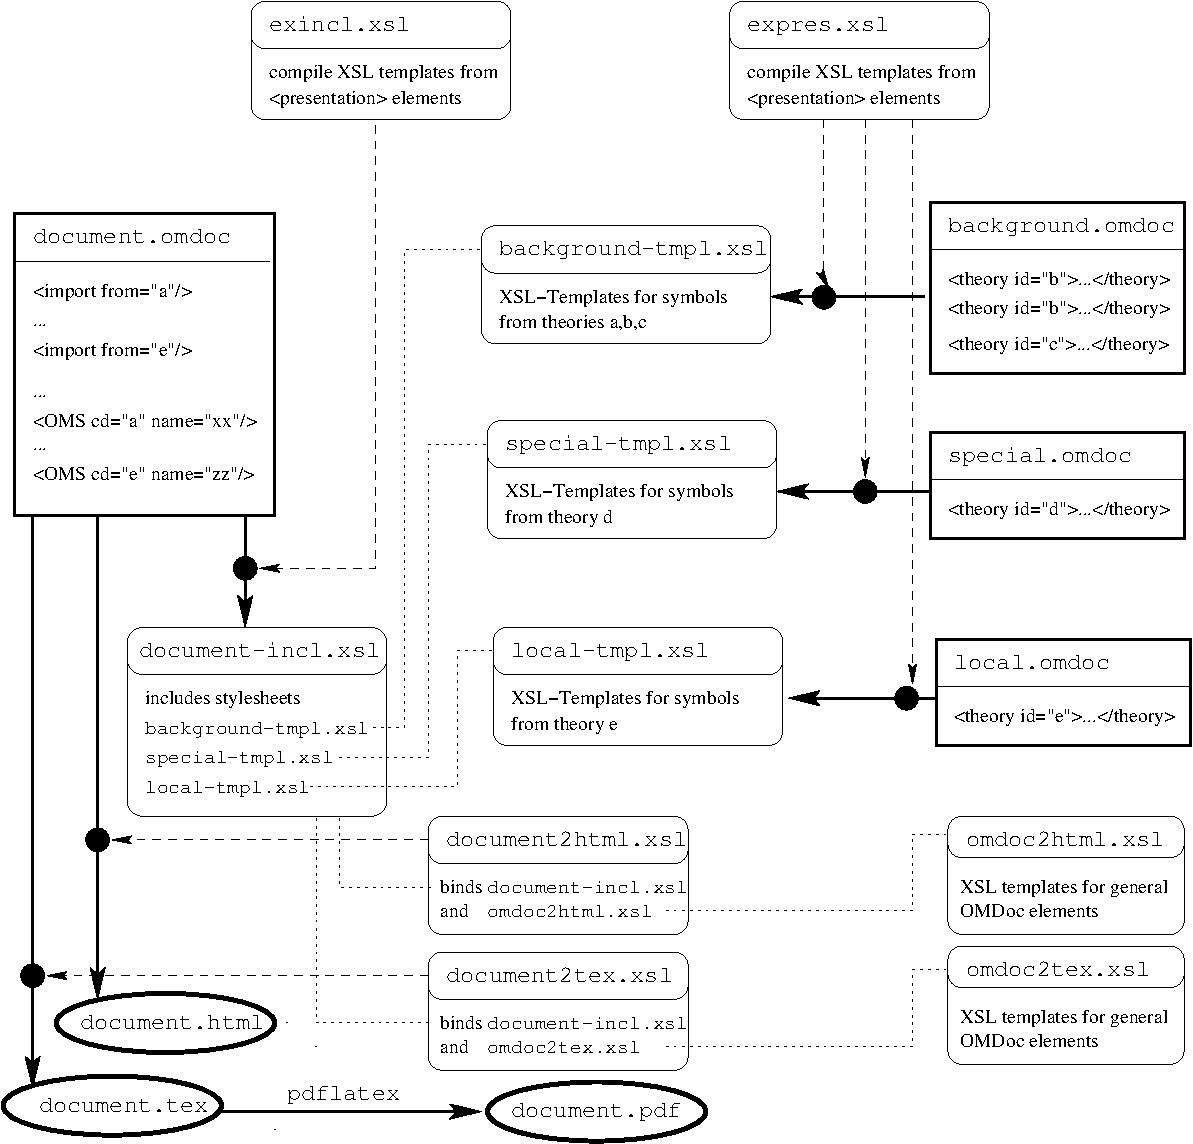
\includegraphics[width=10.5cm]{figures/presentation-arch}
\end{myfig}

Other processing architectures may be built up using
on-demand technologies, e.g. servlets, mediators, or web services, but will be
able to follow the same general pattern as our simpleminded implementation in
{\snippet{Makefiles}}.

We will make use of this general architecture based on extraction and linking via
{\xslt} style sheets in the transformation of {\omdoc} documents below.


\end{tsection}

\begin{tsection}[id=omdoctosys,short=Interfaces for Systems]{{\omdoc} Interfaces for Mathematical Software Systems}

  One of the original goals of the {\openmath}, {\cmathml} and {\omdoc} languages is to
  provide a communication language for mathematical software systems. The main idea behind
  this is to supply systems with interfaces to a universally accepted communication
  language standard (an {\indextoo{interlingua}}), and so achieve interoperability for $n$
  systems with only $2n$ translations instead of $n^2$. As we have seen in
  {\mysecref{math-objects}}, {\openmath} and {\cmathml} provide a good solution at the
  level of mathematical objects, which is sufficient for systems like {\twintoo{computer
      algebra}{system}s}. {\omdoc} adds the level of mathematical statements and theories
  to add support for automated reasoning systems and formal specification systems.

To make practical use of the {\omdoc} format as an interlingua, we have to support
building {\omdoc} interfaces. An {\xslt} style sheet is a simple way to come up with (the
input half) of an {\omdoc} interface.  A more efficient way would be to integrate an
{\xml}\twin{XML}{parser} directly into the system (suitable {\xml} parsers are readily
available for almost all programming languages nowadays).

Usually, the task of writing an {\xslt} style sheet for such a conversion is a
relatively simple task, since the input language of most mathematical software
system is isomorphic to a subset of {\omdoc}. This suggests the general strategy
of applying the necessary syntax transformations (this has to be supplied by the
style sheet author) on those {\omdoc} elements that carry system-relevant
information and transforming those that are not (e.g. Metadata and {\element{CMP}}
elements for most systems) into comments.  Much of the functionality is already
supplied by the style sheet {\snippetin{omdoc2sys.xsl}}, which need only be adapted to
know about the comment syntax. 

The task of translating an {\omdoc} document into system-specific input has two
sub-tasks. We will discuss them using the concrete example of the
{\snippetin{omdoc2pvs.xsl}} style sheet that transforms {\omdoc} documents to the input
language of the {\pvs} theorem prover~\cite{OwRu92}: The first task is to translate
elements at the statement- and theory level to the input language this is hand-coded by
supplying suitable templates for the {\omdoc} statement and theory elements in an
extension of the {\snippet{omdoc2sys.xsl}} style sheet. The second task is to translate
the formulae to the input language. Here, the system usually has a particular way of
expressing complex formulae like function applications and binding expressions; in the
concrete case of {\pvs}, function application uses a prefix function argument syntax, and
$n$-ary binding expressions, where the scope is separated by a colon from the variable
list. This information must also be encoded in respective templates for the
{\element[ns-elt=om]{OMA}}, {\element[ns-elt=om]{OMBIND}}, {\element[ns-elt=om]{OMV}}
elements from {\openmath} and the {\element[ns-elt=m]{apply}} and {\element[ns-elt=m]{ci}}
from {\cmathml}. For the symbol elements, we have to distinguish two cases: the
{\twintoo{predefined}{symbol}s} of the system language and the {\twintoo{object}{symbol}s}
that are introduced by the user to formalize a certain problem. In both cases, the
transformation procedure needs input on how these symbols are to be represented in the
system language. For the {\twintoo{object}{symbol}s} we assume that there are suitable
{\element{theory}} structures available, which declare them in {\element{symbol}}
elements, thus we can assume that these {\element{theory}} structures also contain
{\element{use}} elements with appropriate {\attribute{format}{use}} attribute in the
{\element{presentation}} elements for those symbols that need special representations in
the system language.  For the {\twintoo{predefined}{symbol}s} of the system language, we
assume the same.  To be able to transform an {\omdoc} document into system input, we need
a {\twintoo{language definition}{theory}}, i.e. an {\omdoc} document that contains a
{\element{theory}} which provides {\element{symbol}s} for all the predefined words of the
system language. This theory must also contain {\element{presentation}} elements with
{\element{use}} children specialized the input formats of all systems targeted for
communication.

\begin{lstlisting}[label=lst:system-language,
  caption={A {\element{symbol}} in a Language Definition Theory},
  index={symbol,presentation,style}]
<symbol name="sigmatype">
 <metadata>
   <dc:description>
     The dependent function type constructor is a binding operator. The source type is
     the type of the bound variable X, the target type is represented in the body.
   </dc:description>
 </metadata>
</symbol>

<presentation xml:id="pr-sigmatype" for="#sigmatype" role="binding">
  <style format="pvs">
    <text>[</text>
    <recurse select="*[2]/*"/><text> -&gt; </text><recurse select="*[3]"/>
    <text>]</text>
  </style>
  <style format="nuprl">
    <recurse select="*[2]/*"/><text> -&gt; </text><recurse select="*[3]"/>
  </style>
</presentation>
\end{lstlisting}

The other direction of the translation needed for communication is usually much
more complicated, since it involves parsing the often idiosyncratic output of
these systems. A better approach is to write specialized output generators for
these systems that directly generate {\omdoc} representations. This is usually a
rather simple thing to do, if the systems have internal data structures that
provide all the information required in {\omdoc}. It is sometimes a problem with
these systems that they only store the name of a symbol (logical constant) and not
its home theory. At other times, internal records of proofs in theorem provers are
optimized towards speed and not towards expressivity, so that some of the
information that had been discarded has to be recomputed for {\omdoc} output.

One of the practical problems that remains to be solved for interfaces between
mathematical software systems is that of semantic standardization of input
languages. For mathematical objects, this has been solved in principle by supplying a
theory level in the form of {\openmath} or {\omdoc} content dictionaries that define the
necessary mathematical concepts. For systems like theorem provers or theory development
environments we need to do the same with the logics underlying these systems. For an
effort to systematize logics into a hierarchy that fosters reuse and communication of
systems, based on a series of experiments of interfacing with the theorem proving systems
{\OMEGA}~\cite{BenzmuellerEtAl:otama97}, {\inka}~\cite{HuSe:itng96}, {\pvs}~\cite{OwRu92},
{\lambdaclam}~\cite{RicSmaGre:ppihol98}, {\tps}~\cite{AnBi:tatps96} and
{\coq}~\cite{CoqManual} see {\mysecref{logics}}
\end{tsection}

\begin{tsection}[id=omdoc2pres]{Presenting OMDoc to Humans}
We will now discuss the software infrastructure needed to transform {\omdoc}
documents into human-readable form in various formats. We speak of of {\omdoc}
{\defin{presentation}} for this task.

Due to the complex nature of {\omdoc} presentation, only part of it
can actually be performed by {\xslt} style sheets. For instance,
sub-tasks like reasoning about the prior knowledge of the user, or her
experience with certain proof techniques is clearly better left to
specialized applications. Our processing model is the following:
presenting an {\omdoc} is a two-phase process. 

The first phase is independent of the final output format (e.g. {\html}, {\mathml}, or
{\LaTeX}) and produces another {\omdoc} representation specialized to the respective user
or audience, taking into account prior knowledge, structural preferences, bandwidth and
time constraints, etc.  This phase usually generates a
{\twintoo{narrative-structured}{document}} from a knowledge-centered
one\twin{knowledge-centered}{document}. 

The second phase is a formatting process that can be extracted by {\xslt} style sheets
that transforms the resulting specialized document into the respective output format with
notational- and layout preferences of the audience. We will only discuss the second one
and refer the reader for ideas about the first process to systems like
P.rex~\cite{Fiedler:ddaoeo01,FiedlerHoracek:aietlp01}.

The presentation of the {\omdoc} document elements and statements is carried out by the
style sheets {\snippetin{omdoc2html.xsl}} for {\xhtml}, {\snippetin{omdoc2html.xsl}} for
{\xhtml}+{\mathml} and {\snippetin{omdoc2tex.xsl}} for {\LaTeX}. These style sheets are
divided into files according to the {\omdoc} modules and share a large common code base
{\snippetin{omdoc2share.xsl}}, basically the first two include the latter and only
redefine some format-specific options. For instance, {\snippetin{omdoc2share.xsl}}
supplies an infrastructure for {\indextoo{internationalization}} introduced in
{\mysecref{mtext}}. This allows to generate localized presentations of the {\omdoc}
documents, if enough information is present in the
{\twintoo{multilingual}{group}s}\twin{multilingual}{support}\twin{languages}{multiple} of
{\element{CMP}} elements. {\snippetin{omdoc2share.xsl}} takes a {\indextoo{parameter}}
{\snippetin{TargetLanguage}}, whose value can be a whitespace-separated preference list of
{\atwintoo{ISO}{639}{norm}} two-letter {\twintoo{country}{code}s}.  If
{\snippetin{TargetLanguage}} consists of a single entry, then the result will only contain
this language with gaps where the source document contains no suitable {\element{CMP}}.
Longer {\snippetin{TargetLanguage}} preference lists will generally result in more
complete, but {\twintoo{multilingual}{document}s}. Apart from the language-specific
elements in the source document, {\indextoo{localization}} also needs to know about the
presentation of certain keywords used in {\omdoc} markup, e.g.  the German ``Lemma'' and
the French ``Lemme'' for {\snippet{<assertion type="lemma">}}. This information is kept in
the keyword table {\snippet{lib/locale.xml}} in the {\omdoc} distribution, which contains
all the keywords necessary for presenting the {\omdoc} elements discussed so far.  An
alternative keyword table can be specified by the parameter {\index{parameter!{\xslt}}}
{\snippet{locale}}\index{locale@{\snippet{locale}} ({\xslt} parameter)}.
\end{tsection}
\end{tchapter}
%%% Local Variables: 
%%% mode: latex
%%% TeX-master: "omdoc"
%%% End: 

% LocalWords:  xsl saxon xalan xsltproc internet mozilla netscape cd xslt tmpl
% LocalWords:  expres omstyle ref exincl incl ab pvs rex pmml tex mtext Lemme
% LocalWords:  TargetLanguage ombind fol omdocIhtml xxx testIhtml pres pdflatex
% LocalWords:  ci changelog lib omdoctosys ns elt omdoc html CMP sys ary OMA
% LocalWords:  OMV sigmatype metadata recurse nuprl
